
% The \phantomsection command is needed to create a link to a place in the document that is not a
% figure, equation, table, section, subsection, chapter, etc.
% https://tex.stackexchange.com/questions/44088/when-do-i-need-to-invoke-phantomsection
\phantomsection

% Multiple-language document - babel - selectlanguage vs begin/end{otherlanguage}
% https://tex.stackexchange.com/questions/36526/multiple-language-document-babel-selectlanguage-vs-begin-endotherlanguage
\begin{otherlanguage*}{brazil}

\chapter{\lang{Service}{Serviço}}\label{cap:servico}

Neste capítulo, abordamos a conceituação do nosso serviço de
\textit{Checkpoint/Restore} de contêineres \textit{Stateful} no Kubernetes.
Apresentamos a arquitetura geral do serviço e como os componentes da arquitetura
se comunicam entre si. Também é apresentado as duas implementações que foram
abordadas no trabalho, uma utilizando técnicas de \textit{Event Sourcing} e a
outra utilizando técnicas mais difundidas para \textit{Checkpoint/Restore} através
da utilização de CRIU para salvamento do estado de uma aplicação. Serão apresentados
ao longo do texto diagramas de sequência que representam o funcionamento da
arquitetura.

\section{Arquitetura Geral}

A arquitetura do serviço possibilita o \textit{Checkpoint/Restore} transparente das
aplicações monitoradas pelo serviço no Kubernetes. Esta arquitetura é agnóstica sobre
a implantação, seja ela em Kubernetes ou localmente em um sistema, é fortemente inspirada
pelo trabalho em \cite{muller2022architecture}. A arquitetura é possível de implementar
de diferentes formas, como na utilização de CRIU quanto de técnicas de
\textit{Event Sourcing}. Esta arquitetura também é adequada para execução em
\textit{cluster} de máquinas e adequada para microsserviços \citep{vayghan2021kubernetes}
\cite{muller2022architecture} \cite{oh2018stateful}, embora ainda falte um pouco de
compreensão de como poderemos utilizar ela em sistemas distribuídos geograficamente
de forma eficiente.

\subsection{Checkpoint/Restore}

O \textit{Checkpoint/Restore} de aplicações \textit{stateful} em contêineres podem ser
feitas entre duas formas, como abordamos no \ref{cap:fundamentacao:teorica}, ou
utilizando técnicas de salvamento do contexto dos processos, com isolação do contexto
provida para contêineres \cite{muller2022architecture} com CRIU, ou com as técnicas de
\textit{Event Sourcing}. No nosso serviço a parte de recuperação dos estados será
administrada pelo componente de Administrador de Estado, já a parte de salvamento de estado
será feita ativamente pelo Interceptador. Juntos estes dois componentes fornecem a
funcionalidade de salvamento do estado da aplicação e posterior recuperação em caso
de falhas.

\subsection{Armazenamento}

Para realizar os salvamentos de estados pelo Interceptador, é interessante que eles sejam
feitos de forma periódica, capturando o estado da aplicação em determinado ponto da execução.
Desta forma, é necessário armazenar este estado em algum armazenamento, podemos utilizar. Para
isso teremos a imagem gerada por \textit{Checkpoint} que deverá ser armazenada em algum lugar
para ser posteriormente recuperada, em \cite{vayghan2021kubernetes} utiliza-se o conceito de
volumes para armazenamento dos dados, aqui também iremos utilizar o mesmo conceito, tanto para
imagens de \textit{Checkpoint} quanto para armazenamento de eventos.

Ainda na questão do armazenamento, para utilização de \textit{Checkpoint} com CRIU,
diferentemente do \textit{Event Sourcing} é interessante sabermos metadados sobre o momento
de salvamento da imagem, que nos ajudem a identificá-la no tempo \cite{oh2018stateful}
\cite{muller2022architecture} \cite{Chen2015/10}. Para isso, nos trabalhos de
\cite{muller2022architecture}, \cite{oh2018stateful} e \cite{Chen2015/10} utilizou-se
bancos de dados distribuídos de chave/valor como o etcd. Nosso administrador de estado também
utilizará o mesmo conceito para armazenar metadados das imagens.

\subsection{Recuperação ao último estado}

Durante um salvamento do estado da aplicação a aplicação permanece indisponível para
servir requisições e comandos do usuário, pois, as técnicas de salvamento de estado
de contêineres com CRIU congelam o processo da aplicação para salvar o estado
\cite{vayghan2021kubernetes}. Já no \textit{Event Sourcing} não possuimos este problema.
Entretanto, no segundo caso precisamos saber a ordem em que as requisições chegam para
podermos reprojetar o estado da aplicação a partir da reemissão das requisições à aplicação
monitorada. Ainda no caso do CRIU, ainda precisamos saber quais as requisições que chegaram
a partir de um salvamento de estado, já que todas requisições posteriores àquele salvamento
não estaram no estado salvo, precisaremos replicá-las para o serviço monitorado também. De
modo geral, o que temos de diferença é que no caso do CRIU reprojetamos apenas as requisições
a partir do último ponto de salvamento, já no caso do \textit{Event Sourcing} replicamos
as requisições desde o começo da existência da aplicação.

Para solucionar o problema de alcançar o último estado possível da aplicação em uma
recuperação para nossos dois casos, iremos utilizar no nosso Interceptador o padrão de projeto
de Embaixador(\textit{Ambassador}) como em \cite{muller2022architecture}. Nosso Interceptador
irá interceptar as requisições que chegam a nossa aplicação monitorada, irá salvar cada uma
das requisições em um volume, que pode ser em memória ou armazenamento persistente, e
encaminhá-las a aplicação. Sempre que formos realizar uma restauração iremos replicar as
requisições a partir do último ponto de salvamento para utilização de CRIU, como em 
\cite{muller2022architecture}, mas, no caso do \textit{Event Sourcing} faremos uma
reprojeção total com todas as requisições feitas desde o momento que a aplicação começou a
executar.

Para que novas requisições que chegarem durante o processo de restauração não interfiram na
ordem do estado com as requisições sendo refeitas. Nosso Interceptador tem dois estados de
operação um Ativo que está enviando requisições diretamente para a aplicação monitorada, e
outro de Aguardo que ficará esperando a restauração terminar para começar a enviar as
requisições, neste estado as requisições não serão respondidas imediatamente aos clientes,
mas, só após a restauração finalizar, quando o estado do Interceptador retornar para Ativo.
Em \cite{vayghan2021kubernetes} algo semelhante foi feito sobre estados da aplicação sendo
recuperada para impedir que requisições cheguem com estado desatualizado da aplicação.


\subsection{A Arquitetura}

As subseções acima trouxeram um pocuo dos problemas que temos que enfrentar e como
resolvemos cada um dos problemas com algum componente do sistema. Nesta subseção, iremos
abordar um pouco de como os componentes se comunicam entre a arquitetura e delimitar as
funcionalidades de cada um dos componentes sem abordar nenhum tipo de implementação
específica. Aqui, abordamos o que o Administrador de Estado, o Interceptador, o Volume, o
Banco de dados e Conêiner são e fazem. A arquitetura de maneira geral está apresentada na Figura
\ref{fig:abstract-architecture}, e a chamamos de representação geral abstrata da arquitetura.

\begin{figure}[h]
\centering
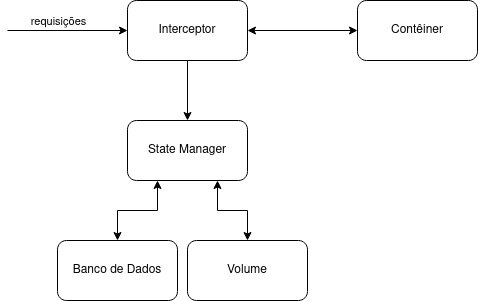
\includegraphics[scale=0.54]{images/abstract-architecture.png}
\caption{Representação da arquitetura abstrata da solução representada através de seus componentes.}
\label{fig:abstract-architecture}
\end{figure}

O Contêiner é a abstração da nossa aplicação com estado, que é o cerne deste trabalho
prover tolerância a falha a contêineres através de \textit{Checkpoint/Restore}. Este Contêiner
contem uma imagem executando, onde o endereçamento de memória é importante para o contexto
de execução da aplicação \cite{Chen2015/10}. A aplicação neste caso pode ser um banco
de dados como Redis ou uma aplicação de \textit{streaming} de vídeo como usado em \cite{vayghan2021kubernetes}.

O Volume é a abstração de um armazenamento persistente ou não para armazenar as imagens e
dados da aplicação. Para o nosso serviço é interessante que este Volume seja acessível
por diversas máquinas em diferentes localidades \cite{vayghan2021kubernetes}, pelo foco
do trabalho em \textit{clusters} de máquinas. Este volume deve permitir escritas das imagens
e recuperação das imagens através de uma interface de acesso.

O Banco de Dados é abstração de um banco de dados específico, este banco de dados precisa
persistir os dados, possibilitar a escrita, leitura e atualização dos dados. Ele também
deve ser distribuído pelo \textit{cluster} e tolerante a falhas para que todos as instâncias
dele consigam servir as mesmas informações consistentemente.

O Interceptor é a nossa aplicação do padrão de projeto do Embaixador \cite{ambassador}. Ele
deve interceptar as requisições a nossa aplicação, enviá-las ao Contêiner, esperar a resposta
deste, salvar a requisição para posterior recuperação das requisições respondidas pelo
Contêiner e responder para o cliente da requisição. Outro requisito do Interceptor é que ele
consiga replicar as requisições a um Contêiner a partir de uma informação de tempo, para que
possamos recuperar um estado do Contêiner apenas repetindo as requisições. O Interceptor também
é o responsável por realizar o salvamento do estado em uma imagem do Contêiner e enviar ao
Administrador de Estado os metadados da última requisição tratada, enquanto se faz um salvamento
também devemos colocar as requisições que chegarem em um \textit{buffer}, a partir da informação
do estado do Interceptador como Aguardo.

Por fim, o Administrador de Estado é o coordenador de toda a operação de
\textit{Checkpoint/Restore}, ele é quem deve receber metadados sobre a aplicação que tem salvamento
de estado feito. Também é o Administrador de Estados que realiza a principal funcionalidade sobre
o processo de restauração que é a identificação da falha do Contêiner monitorado e a atividade de
recuperação pela comunicação com o Interceptador.

\section{Arquitetura com Kubernetes} \label{subsection:kubernetes-architecture}

Para estruturação da arquitetura proposta na Subseção passada no Kubernetes devemos
fazer algumas modificações. Iremos primeiro revisar alguns conceitos abordados no
Capítulo \ref{cap:fundamentacao:teorica}. No Kubernetes temos o conceito de Operator,
eles permitem estender as funcionalidades do Kubernetes, aliados com a API do
Kubernetes podemos monitorar eventos no estado dos recursos e agir de acordo com isso.
Já sabemos que toda aplicação no Kubernetes executa através de um Pod, e, a forma de
realizar a criação e administração de um Pod é através de Deployments e ReplicaSets,
podemos monitorar estes recursos para criar novos Pods e verificar a falha deles.
Também temos PersistentVolumes no Kubernetes que são acessíveis através de todo o
\textit{cluster} e o etcd como banco de dados de chave/valor distribuído disponível
no Kubernetes. Representamos a arquitetura em Kubernetes na Figura
\ref{fig:kubernetes-architecture}.

\begin{figure}[h]
\centering
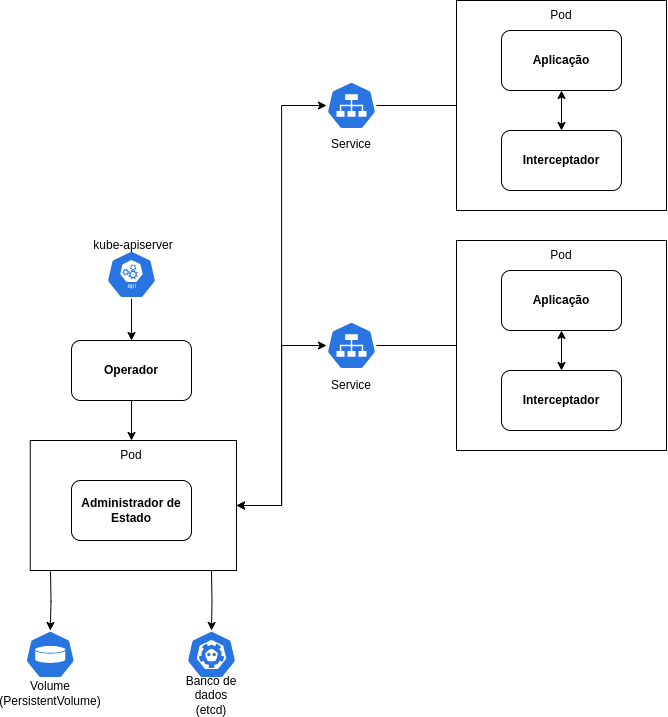
\includegraphics[scale=0.46]{images/kubernetes-architecture.png}
\caption{Representação da arquitetura da solução no Kubernetes.}
\label{fig:kubernetes-architecture}
\end{figure}

O Contêiner da aplicação será implantado a partir de um Deployment do Kubernetes, isto
permite definir a aplicação para ser administrada pelo Deployment usando ReplicaSets.
Com isto, teremos a distribuição do serviço e conseguiremos monitorar a criação, deleção
e atualização dos Pods que o Deployment e o ReplicaSet monitoram através da API do
Kubernetes. Como em \cite{schmidt2023state}, deveremos monitorar e modificar as
funcionalidades do ReplicaSet para possibilitar que nós possamos iniciar novos Pods
da aplicação com imagens recuperadas e identificar quais Pods devemos monitorar com
o nosso Interceptador.

Para implementação do Admnistrador de Estado iremos utilizar também o conceito de Operator
no Kubernetes. O nosso Administrador de Estado será implantado através de um controlador do
estado dos Pods, estes Pods sempre que tiverem uma alteração no seu estado como a falha, iremos
realizar a recuperação do estado. O administrador irá se comunicar com o Interceptador através
do endereço IP do Pod do Kubernetes que pode ser obitdo a partir do momento em que o Pod está
executando e pronto.

Nosso Interceptador será implantado através de um \textit{sidecar container} na aplicação
monitorada, teremos um Operador do Kubernetes que tentará conciliar o estado dos Deployments,
sempre que houver um Deployment com uma anotação do tipo \texttt{crsc.io/checkpoint-restore}
com valor de \textit{true}, iremos criar um novo contêiner no deployment que servirá como 
Interceptador e irá interceptar o tráfego ao Pod. Assim, como em \cite{muller2022architecture},
nosso Interceptador implementado como um \textit{sidecar} permite economia de tráfego, já que
ambos os contêineres operando no Pod tem a mesma interface de rede.

Para o Interceptor é importante que alguns fluxos estejam declarados. Temos o fluxo de
interceptação das requisições, que é representado através de um diagrama de sequência na
Figura \ref{fig:interceptor-request-interception}. Neste diagrama representamos a chegada
de requisições de um usuário até o Interceptor, este salva a requisição em \textit{buffer} para
o passo de reenvio numa restauração e, posteriormente, encaminha as requisições à aplicação,
que, então, serão processadas e uma resposta será enviada ao Interceptor. A resposta
recebida pelo Interceptor permitirá sabermos que o estado foi efetivamente atualizado
na aplicação, marcando a requisição como processada no Interceptor e enviando a resposta ao
usuário que a solicitou.

\begin{figure}[h]
\centering
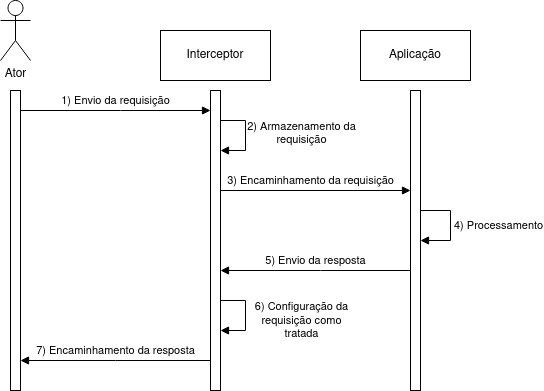
\includegraphics[scale=0.64]{images/interceptor-intercept.png}
\caption{Diagrama de sequência da interceptação de requisição pelo Interceptor.}
\label{fig:interceptor-request-interception}
\end{figure}

Agora para o fluxo de salvamento de uma imagem do contexto de estado da aplicação temos a
Figura \ref{fig:interceptor-checkpoint}. Neste fluxo, temos a comunicação do Interceptador
com o Administrador de Estado. A partir do momento em que o Interceptador percebe que é um
momento para salvamento, seja através de metadados sobre intervalos para coleta, como em \cite{vayghan2021kubernetes}, ou através de detecção de erro como em \cite{tran2022proactive},
ele inicia o fluxo. Inicialmente, todas as requisições param de ser encaminhadas à aplicação
e ficam apenas no \textit{buffer} do Interceptador, este, então, inicia o processo de salvamento
do estado da aplicação utilizando o CRIU. No momento que a imagem estiver pronta, os metadados
dela serão enviados ao Administrador de Estado, que contem principalmente a última requisição
servida, a identificação da aplicação e o horário da imagem. O Administrador de Estado internamente
irá salvar os metadados. Por fim, no Interceptador é retomado o processo de interceptação das
mensagens, servindo as mensagens no \textit{buffer} e reencaminhando novas que chegarem. Em \cite{muller2022architecture} teríamos um passo entre o 5 e o 6, que seria descartar as requisições no \textit{buffer} anteriores a este \textit{checkpoint}, não faremos esta abordagem, manteremos o \textit{buffer} com todas as requisições, salvando-as ou não em um banco de dados persistente, para
que possamos implementar nossa solução específica com técnicas de \textit{Event Sourcing} para
recuperação do estado da aplicação.

As requisições serão mantidas após um \textit{checkpoint}, como mostrado na Figura
\ref{fig:interceptor-checkpoint}, para que seja possível replicá-las a partir de 
ualquer imagem de recuperação ou até mesmo da última imagem possível. Através da
reprojeção das requisições como se fossem eventos, poderemos utilizar o padrão de
projeto de \textit{Event Sourcing} \cite{event-sourcing} para replicar o estado de uma
aplicação até o momento da falha apenas realizando todas as requisições novamente.
Isto poderá ser lento, mas, iremos utilizar esta técnica para comparar com a perda
de latência através de um \textit{checkpoint}, que precisa parar todas as requisições
momentaneamente.

\begin{figure}[h]
\centering
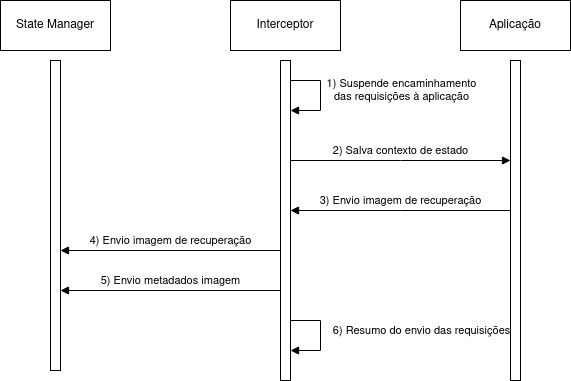
\includegraphics[scale=0.64]{images/interceptor-checkpoint.png}
\caption{Diagrama de sequência do salvamento de imagem feito pelo Interceptor.}
\label{fig:interceptor-checkpoint}
\end{figure}

Já para nossos Volumes para armazenamento persistente das imagens de recuperação
utilizamos os PersistenVolumes do Kubernetes, que possibilitam que os recursos
deste armazenamento persistente sejam acessíveis através de todo o \textit{cluster},
possibilitando que a imagem seja acessível em qualquer nó \cite{kubernetes:persistent-volumes}.
Já para o Banco de Dados utilizamos o etcd que já está presente no Kubernetes, que é
consistente e distribuído entre os nós do Kubernetes, ele permitirá salvar os metadados
das imagens e acessar através de qualquer réplica do State Manager \cite{etcd}
\cite{kubernetes:etcd}.

Por fim, temos o problema de interferir no tráfego da nossa aplicação a ser monitorada.
Conseguimos através da API do Kubernetes e do nosso Operator alterar um Service que iria
indicar o tráfego para o serviço e colocar nosso Interceptador para servir este Service,
pois eles funcionam por padrão como balanceadores de carga. Com isso temos a interceptação
através do Interceptador e podemos interromper as requisições à aplicação quando necessário.

\end{otherlanguage*}
